\begin{figure}[t]
    \centering
    \resizebox{\textwidth}{!}{%
    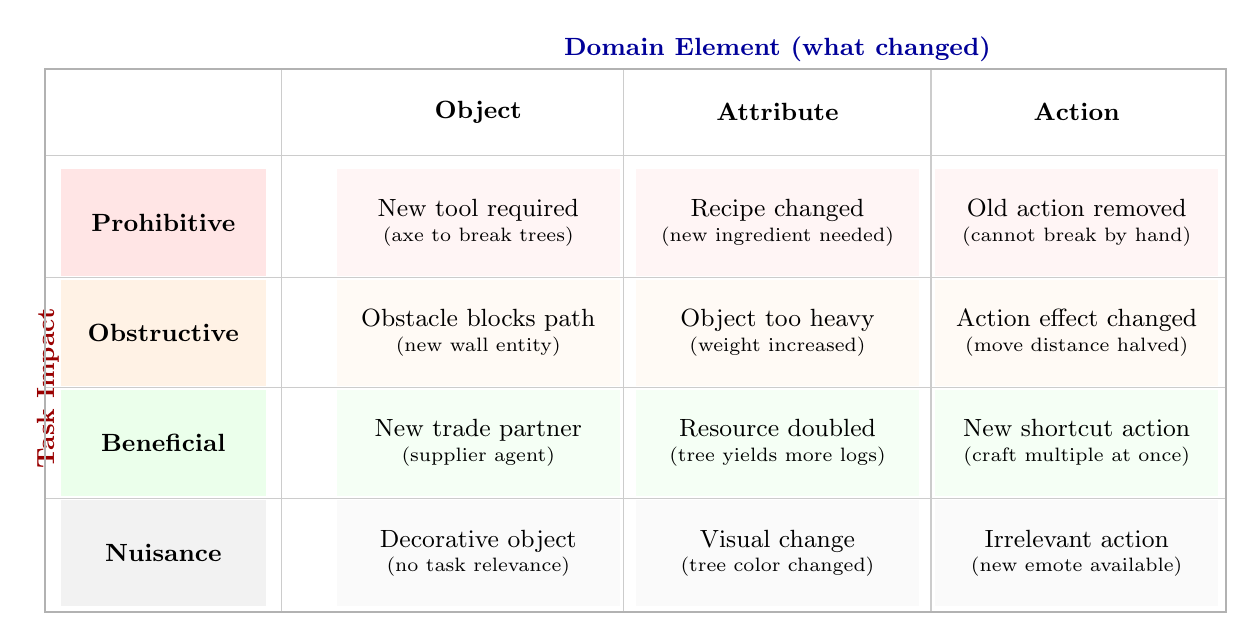
\begin{tikzpicture}[
        % --- Cell styles ---
        cell/.style={
            minimum width=3.6cm, minimum height=1.35cm, 
            align=center, font=\small, inner sep=4pt
        },
        header/.style={
            minimum width=3.6cm, minimum height=0.8cm, 
            align=center, font=\small\bfseries
        },
        rowhead/.style={
            minimum width=2.6cm, minimum height=1.35cm, 
            align=center, font=\small\bfseries
        },
        axislabel/.style={font=\small\bfseries},
    ]

    % ===== Column positions =====
    %  Row headers: x = 0
    %  Col 1 (Object):    x = 4.0
    %  Col 2 (Attribute):  x = 7.8
    %  Col 3 (Action):     x = 11.6

    % ===== Row positions =====
    %  Col headers: y = 0
    %  Row 1 (Prohibitive):  y = -1.4
    %  Row 2 (Obstructive):  y = -2.8
    %  Row 3 (Beneficial):   y = -4.2
    %  Row 4 (Nuisance):     y = -5.6

    % ===== Axis labels =====
    \node[axislabel, text=blue!60!black] at (7.8, 0.8) {Domain Element (what changed)};
    \node[axislabel, text=red!60!black, rotate=90, anchor=south] at (-1.2, -3.5) {Task Impact};

    % ===== Column headers =====
    \node[header] at (4.0, 0.0)  {Object};
    \node[header] at (7.8, 0.0)  {Attribute};
    \node[header] at (11.6, 0.0) {Action};

    % ===== Row headers =====
    \node[rowhead, fill=red!10]    at (0.0, -1.4) {Prohibitive};
    \node[rowhead, fill=orange!10] at (0.0, -2.8) {Obstructive};
    \node[rowhead, fill=green!8]   at (0.0, -4.2) {Beneficial};
    \node[rowhead, fill=gray!10]   at (0.0, -5.6) {Nuisance};

    % ===== Grid lines =====
    % Vertical
    \draw[black!20] (1.5, 0.55) -- (1.5, -6.35);
    \draw[black!20] (5.85, 0.55) -- (5.85, -6.35);
    \draw[black!20] (9.75, 0.55) -- (9.75, -6.35);

    % Horizontal
    \draw[black!20] (-1.5, -0.55) -- (13.5, -0.55);
    \draw[black!20] (-1.5, -2.1) -- (13.5, -2.1);
    \draw[black!20] (-1.5, -3.5) -- (13.5, -3.5);
    \draw[black!20] (-1.5, -4.9) -- (13.5, -4.9);
    \draw[black!20] (-1.5, -6.35) -- (13.5, -6.35);

    % Outer frame
    \draw[black!30, thick] (-1.5, 0.55) rectangle (13.5, -6.35);

    % ===== Prohibitive row =====
    \node[cell, fill=red!4] at (4.0, -1.4)  {New tool required\\[-2pt]{\scriptsize (axe to break trees)}};
    \node[cell, fill=red!4] at (7.8, -1.4)  {Recipe changed\\[-2pt]{\scriptsize (new ingredient needed)}};
    \node[cell, fill=red!4] at (11.6, -1.4) {Old action removed\\[-2pt]{\scriptsize (cannot break by hand)}};

    % ===== Obstructive row =====
    \node[cell, fill=orange!4] at (4.0, -2.8)  {Obstacle blocks path\\[-2pt]{\scriptsize (new wall entity)}};
    \node[cell, fill=orange!4] at (7.8, -2.8)  {Object too heavy\\[-2pt]{\scriptsize (weight increased)}};
    \node[cell, fill=orange!4] at (11.6, -2.8) {Action effect changed\\[-2pt]{\scriptsize (move distance halved)}};

    % ===== Beneficial row =====
    \node[cell, fill=green!4] at (4.0, -4.2)  {New trade partner\\[-2pt]{\scriptsize (supplier agent)}};
    \node[cell, fill=green!4] at (7.8, -4.2)  {Resource doubled\\[-2pt]{\scriptsize (tree yields more logs)}};
    \node[cell, fill=green!4] at (11.6, -4.2) {New shortcut action\\[-2pt]{\scriptsize (craft multiple at once)}};

    % ===== Nuisance row =====
    \node[cell, fill=gray!4] at (4.0, -5.6)  {Decorative object\\[-2pt]{\scriptsize (no task relevance)}};
    \node[cell, fill=gray!4] at (7.8, -5.6)  {Visual change\\[-2pt]{\scriptsize (tree color changed)}};
    \node[cell, fill=gray!4] at (11.6, -5.6) {Irrelevant action\\[-2pt]{\scriptsize (new emote available)}};

    \end{tikzpicture}
    }%
    \caption[Two-dimensional novelty taxonomy]{The two-dimensional novelty taxonomy. Columns classify novelties by the type of domain element affected (object, attribute, or action). Rows classify novelties by their impact on the agent's task performance (prohibitive, obstructive, beneficial, or nuisance). Each cell illustrates the combination with a concrete example from the crafting scenario. Both dimensions are agent-relative: the same environmental change may fall into different categories for different agents depending on their knowledge and current task.}
    \label{fig:novelty_taxonomy}
\end{figure}